\section{Question 1}
\subsection{Équations du mouvement}
Soit le système hamiltonien à deux corps, d'invariant $\Ha (p,q)$ où $p$ est la vitesse de chaque corps et $q$ leur position \footnote{On a évidemment $p(t)$ et $q(t)$. Pour une planète, la composante $p_1$ représente sa vitesse dans la direction "$x$" du plan et la composante $p_2$, sa vitesse dans la direction "$y$" du plan.}. Considérons tout d'abord un système où un des deux corps a une masse beaucoup considérablement plus élevé que l'autre, ce qui le rend statique. On a alors 
$$\Ha (p,q) = \frac{1}{2} p^T p - \frac{1}{||q||_2} . $$
On sait que $\dot{\Ha}(p,q) = 0$ car $\Ha$ est invariant dans le temps.
De plus, comme (par la règle de dérivée en chaîne)
\[
  \dot{\Ha}(p,q) = \fpart{\Ha(p,q)}{p}^T\dot{p} + \fpart{\Ha(p,q)}{q}^T\dot{q},
\]
on doit avoir
\[
  \fpart{\Ha(p,q)}{q}^T\dot{q} + \fpart{\Ha(p,q)}{p}^T\dot{p} = 0.
\]

Les équations
\begin{align*}
  \dot{q} & = \fpart{\Ha(p,q)}{p} & \dot{p} & = -\fpart{\Ha(p,q)}{q}
\end{align*}
donnent
\begin{align*}
  \fpart{\Ha(p,q)}{q}^T\dot{q} + \fpart{\Ha(p,q)}{p}^T\dot{p} & =
  \fpart{\Ha(p,q)}{q}^T\fpart{\Ha(p,q)}{p} - \fpart{\Ha(p,q)}{p}^T\fpart{\Ha(p,q)}{q}\\
  & = 0
\end{align*}
ce qui respecte bien l'invariance temporelle de $\Ha$.

Soient $f_1(q,p)$ et $f_2(q,p)$ tels que
\begin{align*}
  \dot{q} & = f_1(q,p)\\
  \dot{p} & = f_2(q,p),
\end{align*}
on calcule
\begin{align*}
  f_1(q,p) & =  \fpart{\Ha (p,q)}{p}\\
  & =
  \begin{pmatrix}
    \fpart{}{p_1} \left(\frac{1}{2}(p_1^2 + p_2^2) - \frac{1}{\sqrt{q_1^2 + q_2^2}}\right)\\
    \fpart{}{p_2} \left(\frac{1}{2}(p_1^2 + p_2^2) - \frac{1}{\sqrt{q_1^2 + q_2^2}}\right)
  \end{pmatrix}\\
  & =
  \begin{pmatrix}
    p_1\\
    p_2
  \end{pmatrix}\\
  & = p\\
%
  f_2(q,p) & =  -\fpart{\Ha (p,q)}{q}\\
  & =
  -\begin{pmatrix}
    \fpart{}{q_1} \left(\frac{1}{2}(p_1^2 + p_2^2) - \frac{1}{\sqrt{q_1^2 + q_2^2}}\right)\\
    \fpart{}{q_2} \left(\frac{1}{2}(p_1^2 + p_2^2) - \frac{1}{\sqrt{q_1^2 + q_2^2}}\right)
  \end{pmatrix}\\
  & =
  \frac{-1}{2(q_1^2 + q_2^2)^{3/2}}
  \begin{pmatrix}
    2q_1\\
    2q_2
  \end{pmatrix}\\
  & = \frac{-q}{\|q\|_2^3}.
\end{align*}
Les équations du mouvement sont donc données par : 
$$\left\lbrace
\begin{array}{ccc}
\dot{q} &=& p\\
\dot{p} &=&  \frac{-q}{\|q\|_2^3}
\end{array}
\right.$$

\subsection{Description des méthodes numériques}
Nous souhaitons intégrer ces systèmes d'équations différentiels non-linéaires (de forme générale $y'(t) = f(t,y)$, où $y$ désigne aussi bien un scalaire qu'un vecteur) par des méthodes numériques : 
\begin{itemize}
\item la méthode d'Euler explicite, $y_{n+1} = y_n + h f(t,y_n)$
\item la méthode d'Euler implicite, $y_{n+1} = y_n + h f(t,y_{n+1})$ qui demande de résoudre une équation non-linéaire de type $g(y_{n+1})=0$, qu'on résoudra en utilisant la méthode itérative de Newton-Raphson
\item la méthode d'Euler symplectique qui est une combinaison des méthodes d'Euler implicite et explicite (on applique le schéma implicite à une composante de $y$ et un schéma explicite à l'autre). 
\end{itemize}

On remarque que $f_1(q,p) = f_1(p)$ et $f_2(q,p) = f_2(q)$.
On va utiliser cette propriété qui va nous être particulièrement utile pour Euler symplectique.
Pour Euler implicite, on aura besoin de
\begin{align*}
  \fpart{f_1(p)}{p} & = I\\
  \fpart{f_2(q)}{q} & =
  \begin{pmatrix}
    \fpart{}{q_1}\frac{-q_1}{(q_1^2 + q_2^2)^{3/2}} &
    \fpart{}{q_2}\frac{-q_1}{(q_1^2 + q_2^2)^{3/2}}\\
    \fpart{}{q_1}\frac{-q_2}{(q_1^2 + q_2^2)^{3/2}} &
    \fpart{}{q_2}\frac{-q_2}{(q_1^2 + q_2^2)^{3/2}}
  \end{pmatrix}\\
  & =
  -\begin{pmatrix}
    \frac{(q_1^2 + q_2^2)^{3/2} + 3q_1^2(q_1^2 + q_2^2)^{1/2}}{(q_1^2 + q_2^2)^3} &
    \frac{3q_1q_2}{(q_1^2 + q_2^2)^{5/2}}\\
    \frac{3q_1q_2}{(q_1^2 + q_2^2)^{5/2}} &
    \frac{(q_1^2 + q_2^2)^{3/2} + 3q_2^2(q_1^2 + q_2^2)^{1/2}}{(q_1^2 + q_2^2)^3}
  \end{pmatrix}\\
  & =
  -\begin{pmatrix}
    \frac{4q_1^2 + q_2^2}{(q_1^2 + q_2^2)^{5/2}} &
    \frac{3q_1q_2}{(q_1^2 + q_2^2)^{5/2}}\\
    \frac{3q_1q_2}{(q_1^2 + q_2^2)^{5/2}} &
    \frac{q_1^2 + 4q_2^2}{(q_1^2 + q_2^2)^{5/2}}
  \end{pmatrix}\\
  & =
  \frac{-1}{\|q\|_2^{5/2}}
  \begin{pmatrix}
    4q_1^2 + q_2^2 &
    3q_1q_2\\
    3q_1q_2 &
    q_1^2 + 4q_2^2
  \end{pmatrix}
\end{align*}

L'équation que Newton-Raphson devra résoudre à chaque pas est la suivante
\begin{align*}
  q_{k+1} & = q_k + hf_1(p_{k+1})\\
  p_{k+1} & = p_k + hf_2(q_{k+1})
\end{align*}
ou encore
\begin{align*}
  q_k - q_{k+1} + hf_1(p_{k+1}) & = 0\\
  p_k + hf_2(q_{k+1}) - p_{k+1} & = 0
\end{align*}
On doit donc résoudre $g(u) = 0$ où
$u =
\begin{pmatrix}
  q_{k+1}\\
  p_{k+1}
\end{pmatrix}$
et
\[
  g
  \left(
    \begin{pmatrix}
      q_{k+1}\\
      p_{k+1}
    \end{pmatrix}
  \right) =
  \begin{pmatrix}
    q_k - q_{k+1} + hf_1(p_{k+1})\\
    p_k + hf_2(q_{k+1}) - p_{k+1}
  \end{pmatrix}
\]
d'où
\[
  \fpart{g}{u}
  \left(
    \begin{pmatrix}
      q_{k+1}\\
      p_{k+1}
    \end{pmatrix}
  \right) =
  \begin{pmatrix}
    -I & h\fpart{f_1}{p}(p_{k+1})\\
    h\fpart{f_2}{q}(q_{k+1}) & -I
  \end{pmatrix}.
\]
Appliquons a présent ces méthodes sur un cas concret où la planète mobile a comme caractéristiques initiales : $p_0 = \begin{matrix}
0\\
2
\end{matrix}
$ et $q_0 = \begin{matrix}
0.4\\
0
\end{matrix} 
$.\\

\subsection{Comparaison des méthodes numériques}
Nous allons appliquer à ce cas les différentes méthodes d'intégration numérique pour 100 000 pas de temps dont la valeur est $h=5e-4$ (Euler implicite et explicite) ou $h=5e-2$ (Euler symplectique). Les résultats sont donnés à la figure \ref{fig:q1}


\begin{figure}
  \centering
  \begin{subfigure}[b]{0.3\textwidth}
    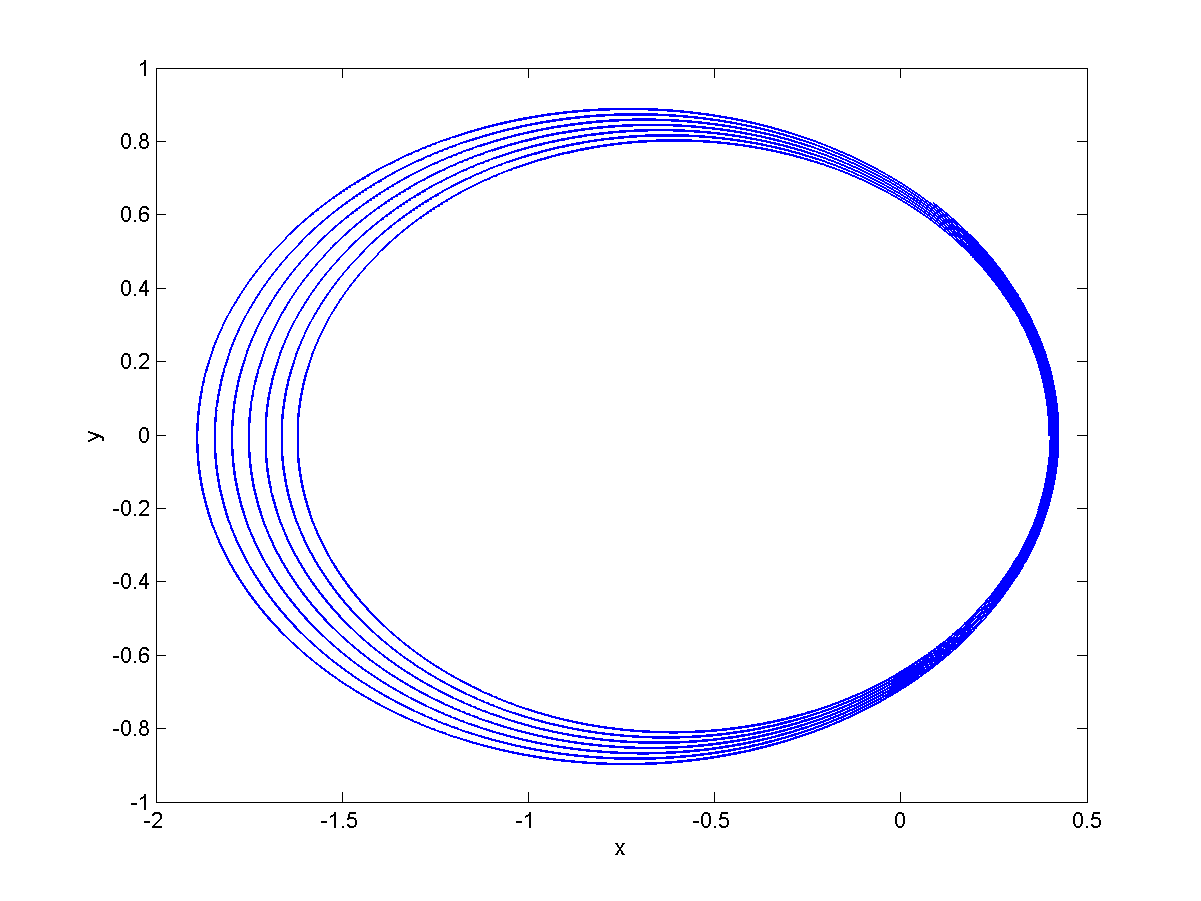
\includegraphics[width=\textwidth]{images/Q1_explicite_q.png}
    \caption{$q$ pour explicite}
    \label{fig:q1_explicite_q}
  \end{subfigure}%
  ~ %add desired spacing between images, e. g. ~, \quad, \qquad etc.
  %(or a blank line to force the subfigure onto a new line)
  \begin{subfigure}[b]{0.3\textwidth}
    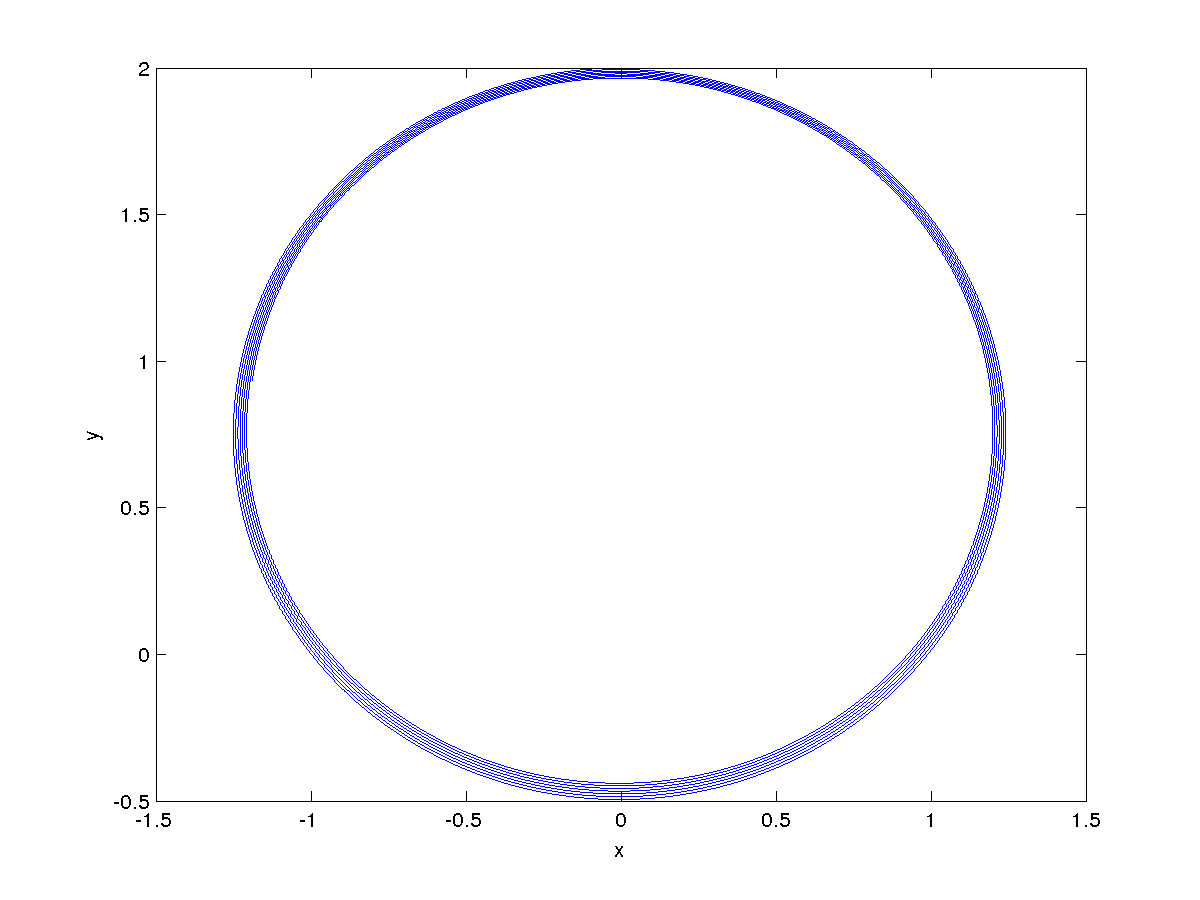
\includegraphics[width=\textwidth]{images/Q1_explicite_p.png}
    \caption{$p$ pour explicite}
    \label{fig:q1_explicite_p}
  \end{subfigure}
  ~
  \begin{subfigure}[b]{0.3\textwidth}
    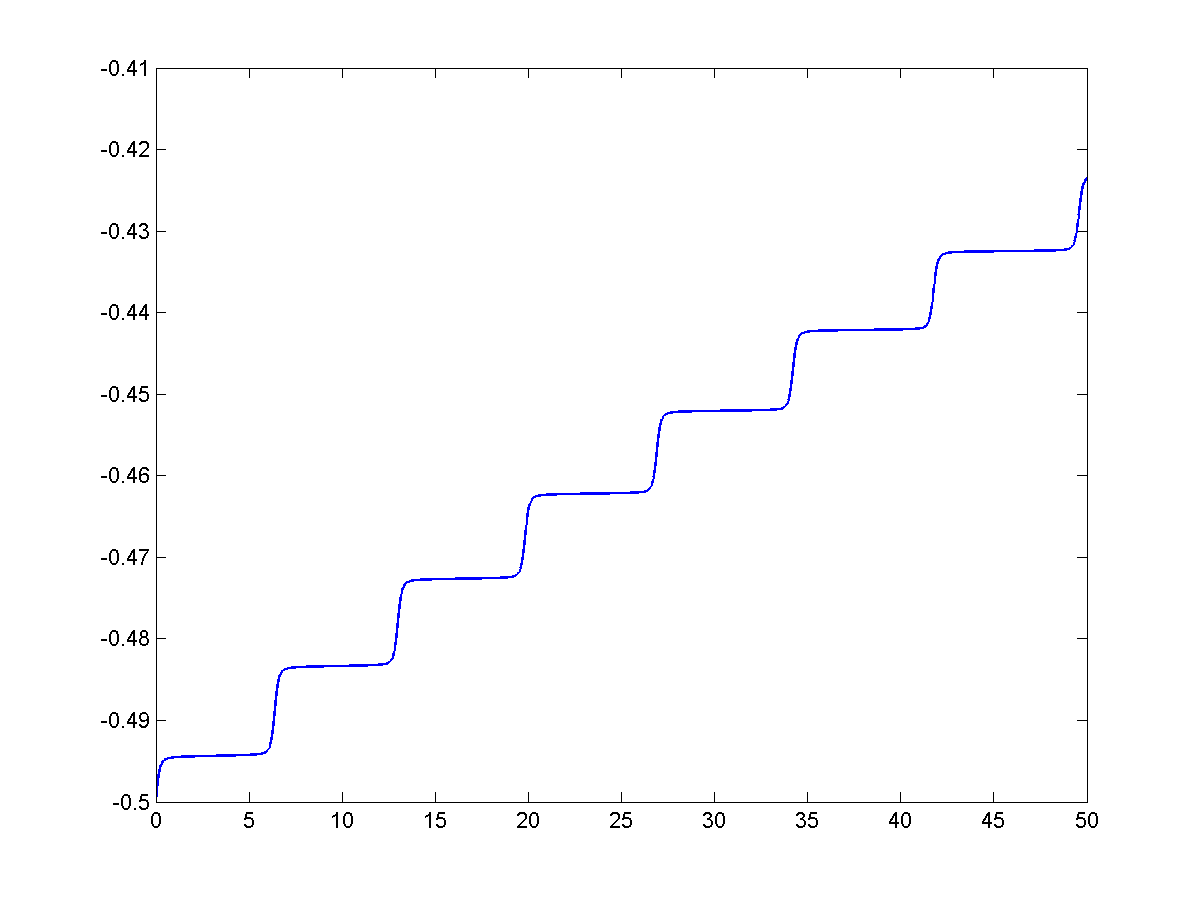
\includegraphics[width=\textwidth]{images/Q1_explicite_H.png}
    \caption{$\Ha$ pour explicite}
    \label{fig:q1_explicite_H}
  \end{subfigure}
  \begin{subfigure}[b]{0.3\textwidth}
    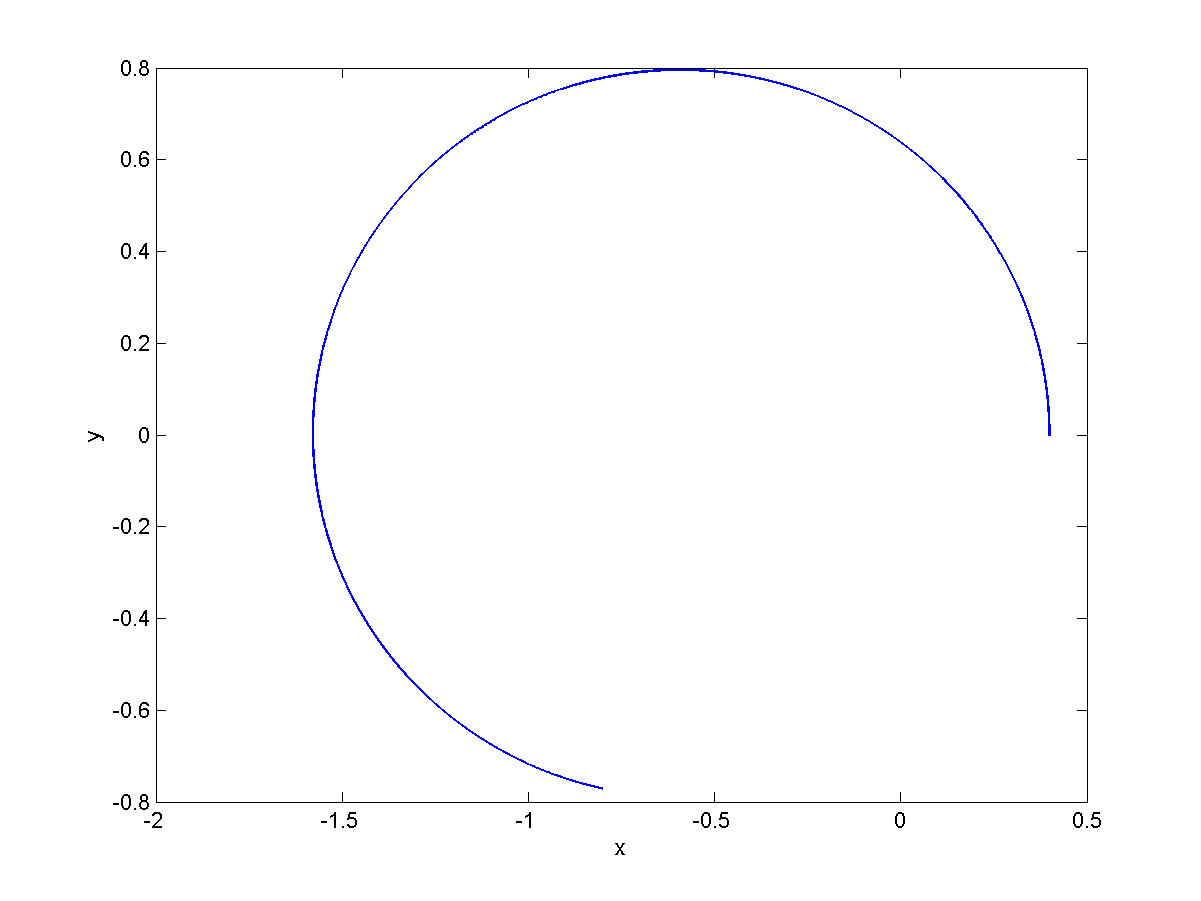
\includegraphics[width=\textwidth]{images/Q1_implicite_q.png}
    \caption{$q$ pour implicite}
    \label{fig:q1_implicite_q}
  \end{subfigure}%
  ~
  %(or a blank line to force the subfigure onto a new line)
  \begin{subfigure}[b]{0.3\textwidth}
    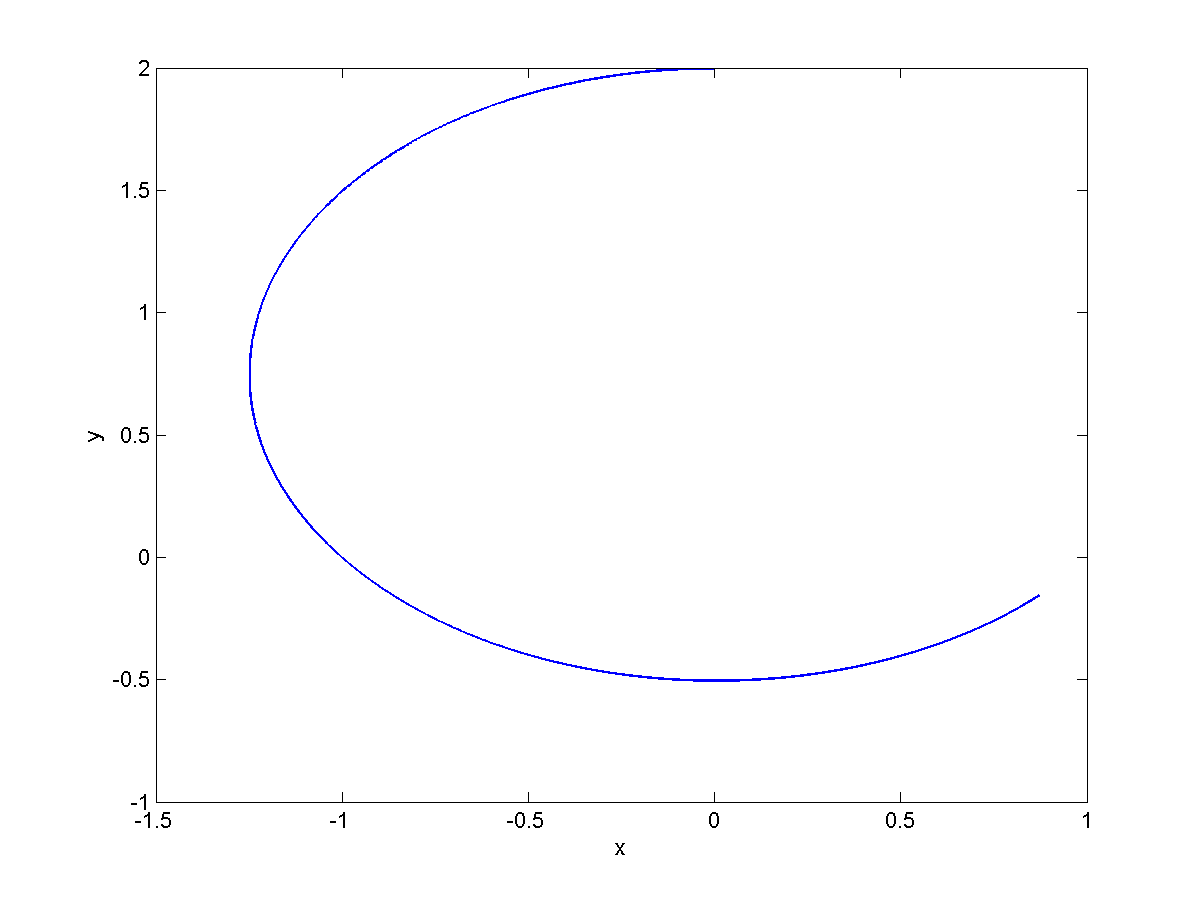
\includegraphics[width=\textwidth]{images/Q1_implicite_p.png}
    \caption{$p$ pour implicite}
    \label{fig:q1_implicite_p}
  \end{subfigure}
  ~
  \begin{subfigure}[b]{0.3\textwidth}
    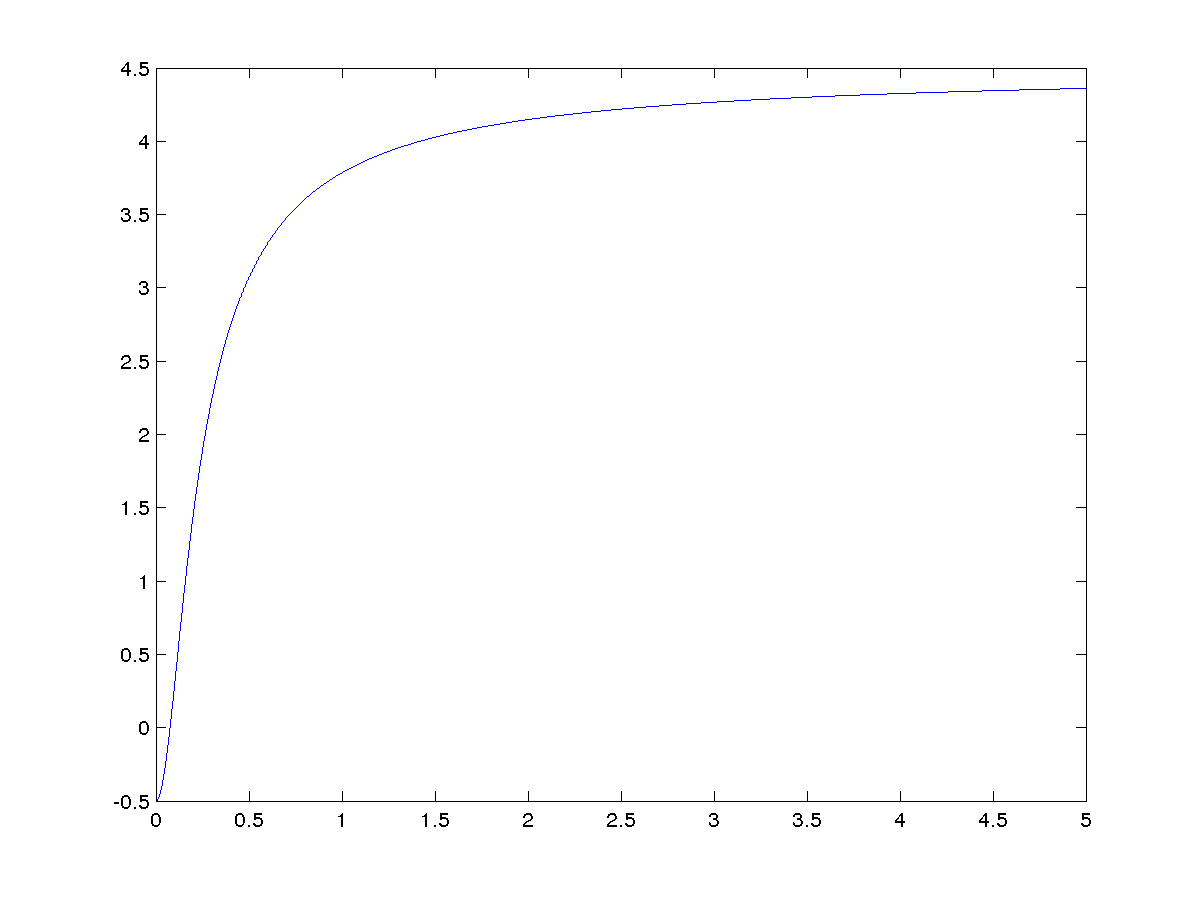
\includegraphics[width=\textwidth]{images/Q1_implicite_H.png}
    \caption{$\Ha$ pour implicite}
    \label{fig:q1_implicite_H}
  \end{subfigure}

  \begin{subfigure}[b]{0.3\textwidth}
    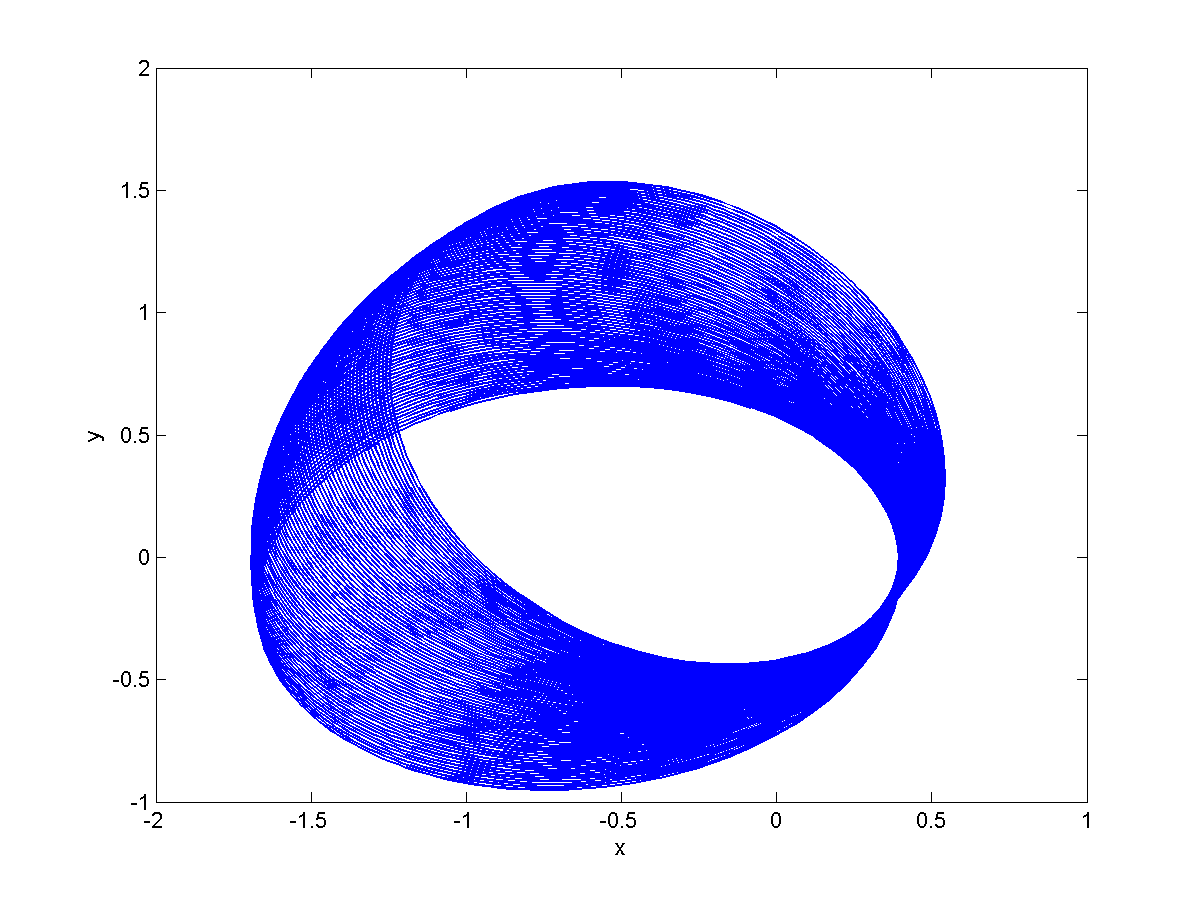
\includegraphics[width=\textwidth]{images/Q1_symplectique1_q.png}
    \caption{$q$ pour symplectique1}
    \label{fig:q1_symplectique1_q}
  \end{subfigure}%
  ~
  %(or a blank line to force the subfigure onto a new line)
  \begin{subfigure}[b]{0.3\textwidth}
    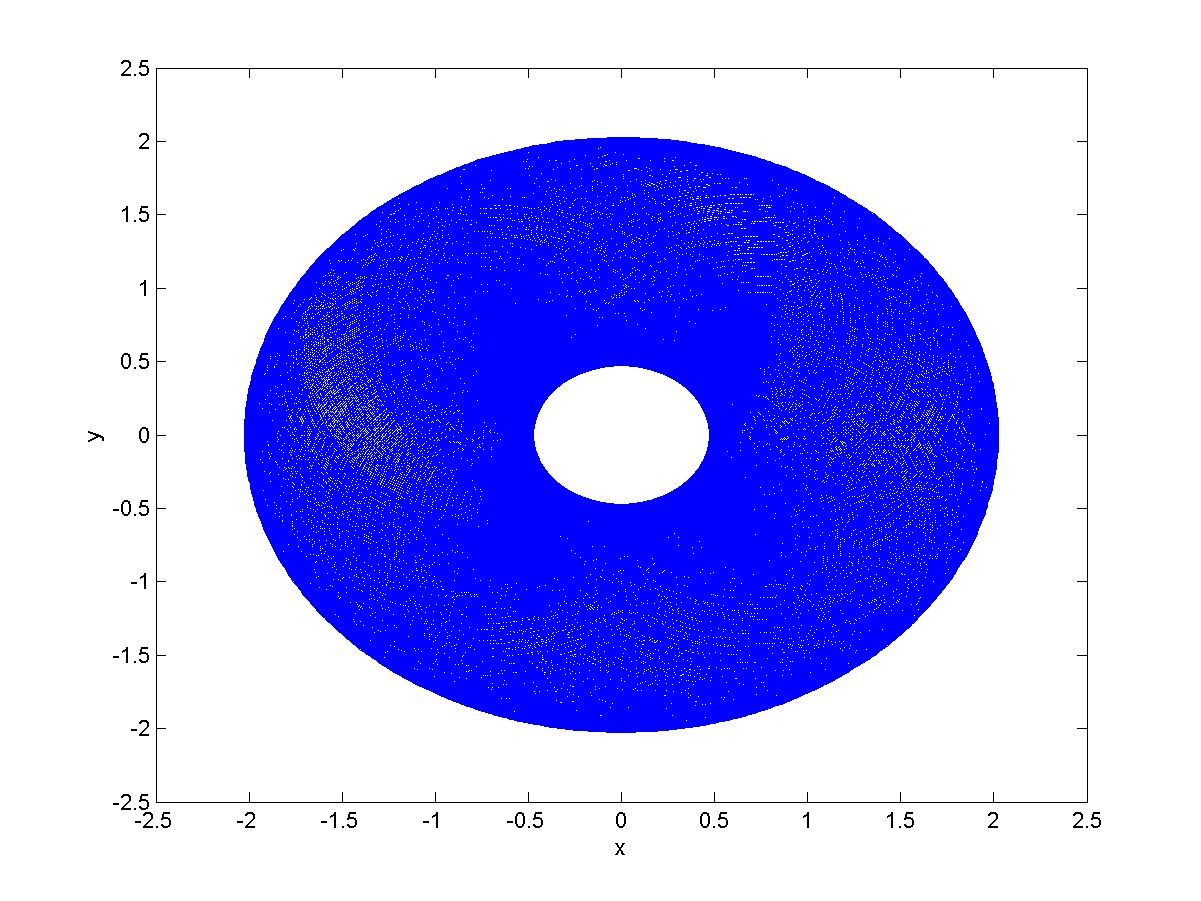
\includegraphics[width=\textwidth]{images/Q1_symplectique1_p.png}
    \caption{$p$ pour symplectique1}
    \label{fig:q1_symplectique1_p}
  \end{subfigure}
  ~
  \begin{subfigure}[b]{0.3\textwidth}
    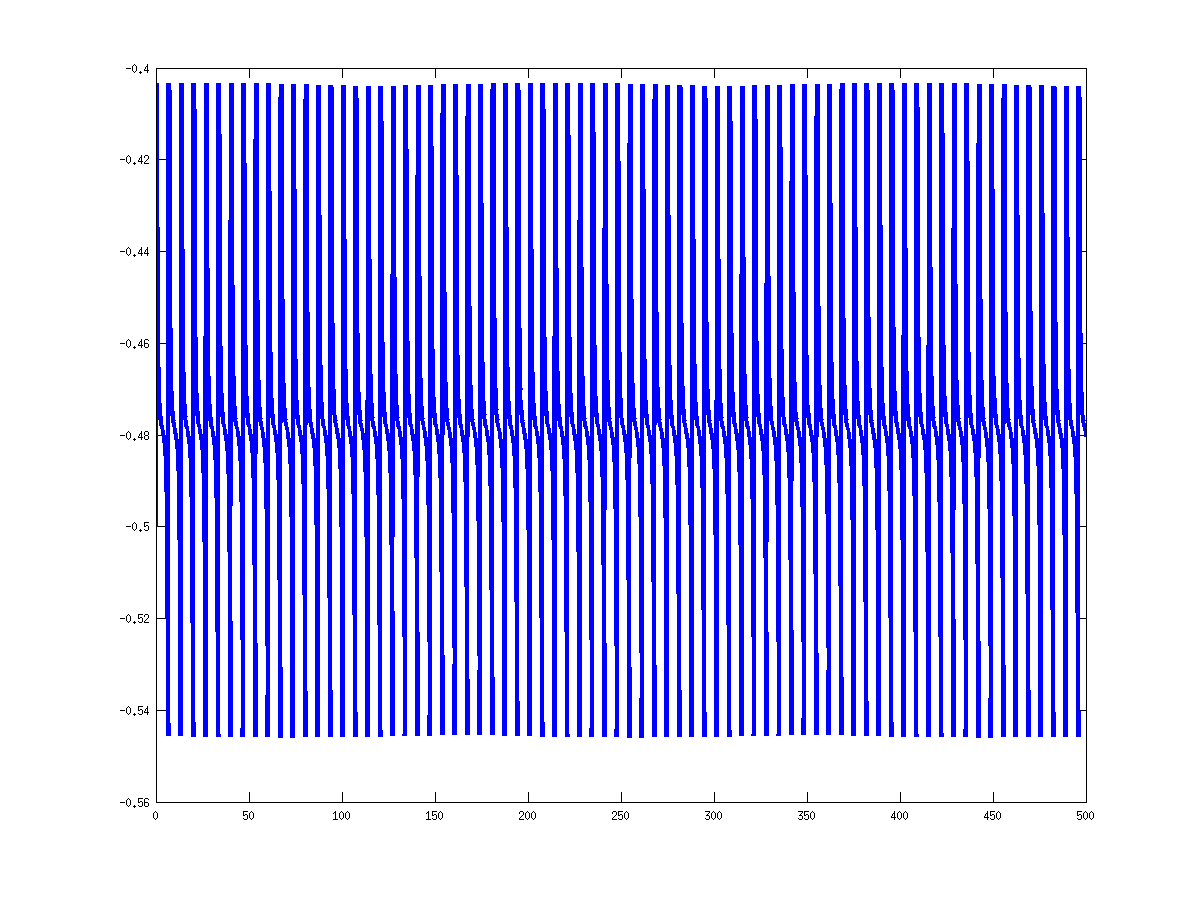
\includegraphics[width=\textwidth]{images/Q1_symplectique1_H.png}
    \caption{$\Ha$ pour symplectique1}
    \label{fig:q1_symplectique1_H}
  \end{subfigure}

  \begin{subfigure}[b]{0.3\textwidth}
    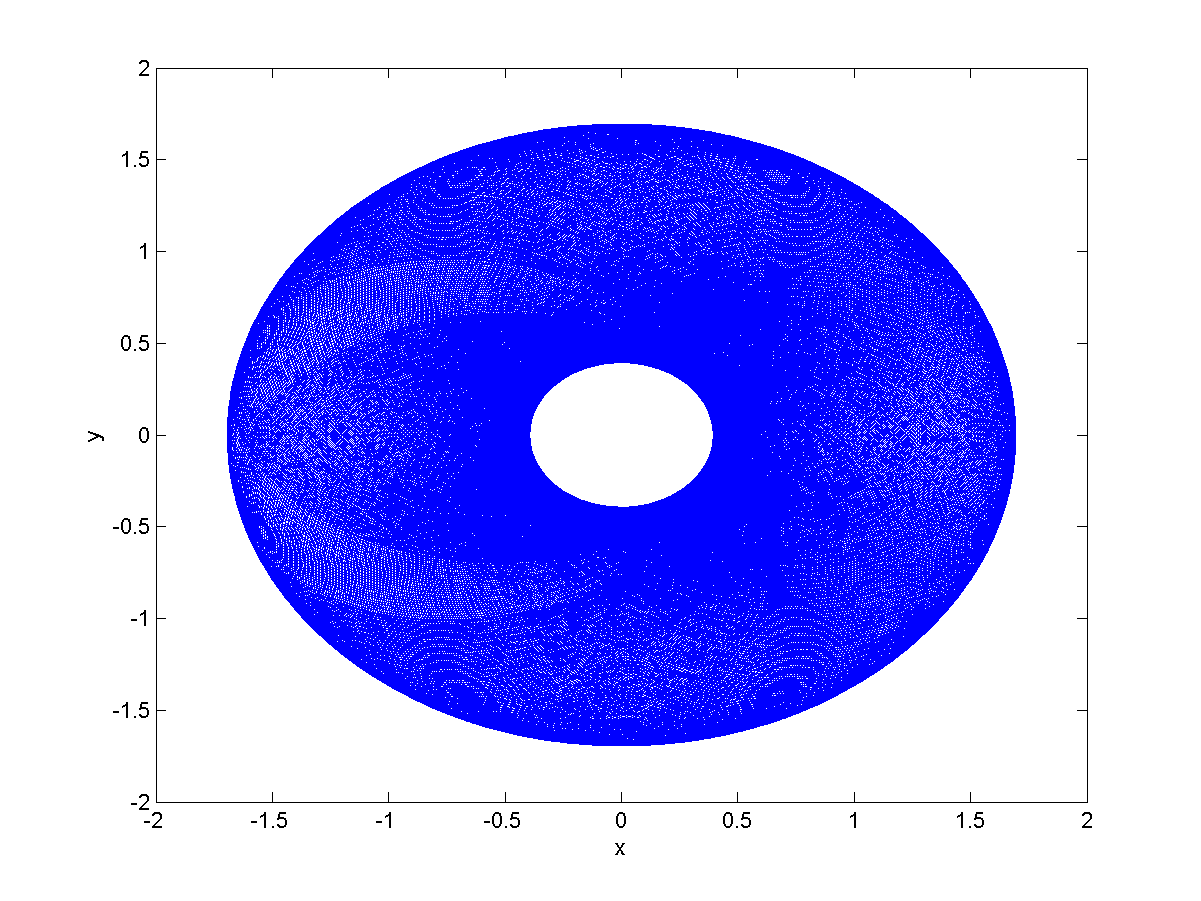
\includegraphics[width=\textwidth]{images/Q1_symplectique2_q.png}
    \caption{$q$ pour symplectique2}
    \label{fig:q1_symplectique2_q}
  \end{subfigure}%
  ~
  %(or a blank line to force the subfigure onto a new line)
  \begin{subfigure}[b]{0.3\textwidth}
    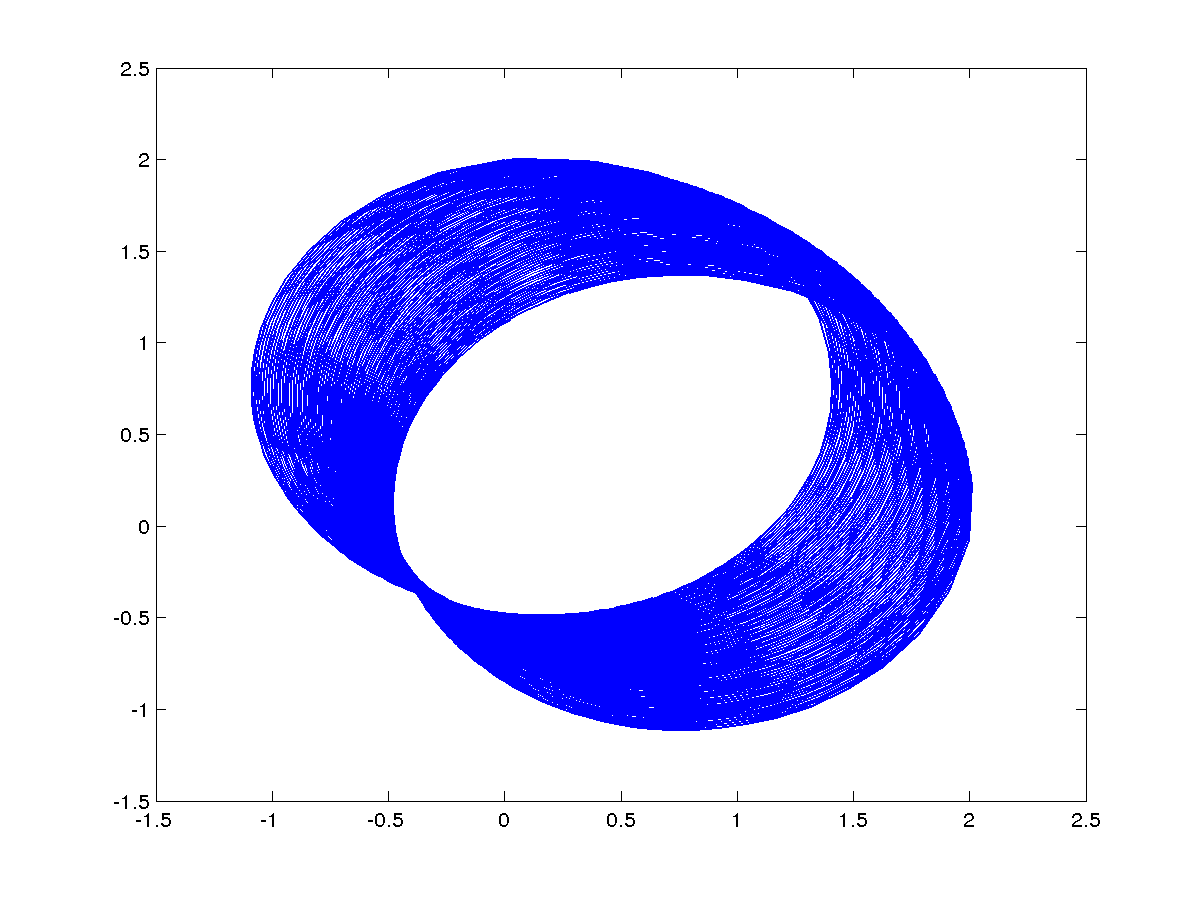
\includegraphics[width=\textwidth]{images/Q1_symplectique2_p.png}
    \caption{$p$ pour symplectique2}
    \label{fig:q1_symplectique2_p}
  \end{subfigure}
  ~
  \begin{subfigure}[b]{0.3\textwidth}
    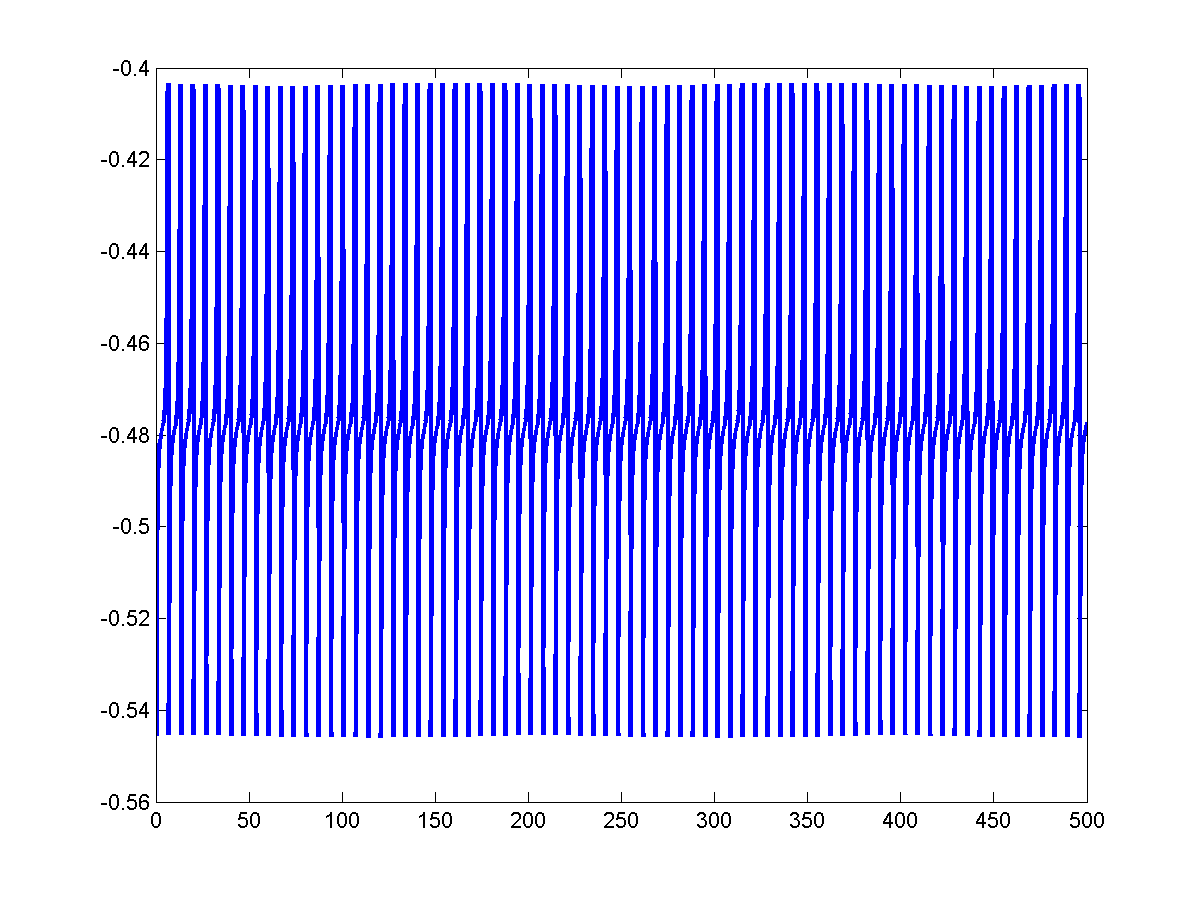
\includegraphics[width=\textwidth]{images/Q1_symplectique2_H.png}
    \caption{$\Ha$ pour symplectique2}
    \label{fig:q1_symplectique2_H}
  \end{subfigure}
  \caption{Résultats pour la question 1}
  \label{fig:q1}
\end{figure}


Les principaux points de comparaison des méthodes sont la convergence, l'erreur et le temps de calcul de la méthode.















